\capitulo{5}{Guante de detección de movimientos involuntarios}

\section{Objetivos}
Uno de los principales inconvenientes de este tipo de patologías es su diagnóstico.
Muchos de estos movimientos son tan imperceptibles o se parecen tanto unos a otros que se hace prácticamente imposible su diagnóstico, impidiendo que los médicos y rehabilitadores sepan con claridad que tipo de tratamiento o terapia seguir y haciendo que su complicada clínica sea aún más difícil.

En un contexto médico donde cada vez se busca más la especialización y la individualización de cada paciente, se ha creado una herramienta que  permitirá obtener datos muy valiosos para ser mucho más específicos en el diagnóstico.

Habiendo explicado todo lo que se sabe a día de hoy sobre los movimientos involuntarios, su principal inconveniente es el diagnóstico, y tras recoger los datos sobre los patrones de movimientos voluntarios e involuntarios mediante la simple prueba del ratón de la aplicación web antes mencionada, se ha conseguido implementar una posible solución para el diagnóstico.

\clearpage

\section{Componentes}

Esta solución consta de un guante el cual hay que modificar con el fin de poder ajustar una serie de sensores situados en una estancia o cubículo que permiten medir el movimiento. Dichos sensores son la clave y el corazón de esta herramienta que a continuación describiremos junto con el resto de componentes:

\begin{itemize}
    \item \textbf{Sensores de distancia ultrasónicos:} Estos se encuentran situados en el cubículo o caja para hacernos más a la idea y permiten conocer la distancia a la que se encuentra la mano de las paredes.
    \item \textbf{Sensor de fuerza:} Permite saber la fuerza que aplica la mano en el guante.
    \item \textbf{Sensor de inclinación:} Nos permite conocer la inclinación que tiene la mano.
    \item \textbf{Arduino:} Es el microcontrolador de la herramienta la cual, nos permite cargar y guardar datos sobre el paciente.
    \item \textbf{Pantalla LCD:} Simplemente es una pantalla que permita al médico ver de manera rápida que sensor es el que está capturando movimientos anómalos.
    \item \textbf{Leds:} Es un refuerzo aun más visual al de la pantalla LCD. 
    \item  \textbf{Protoboards:} La pequeña simula el guante del paciente y la grande seria la caja exterior.
\end{itemize}

\section{Metodología}

Como ya hemos explicado anteriormente esta herramienta es básicamente un guante que consta de una serie de sensores y se encuentra situado en una caja que cuenta con sus propios sensores. 

Gracias a los datos obtenidos de la aplicación anterior, se han trackeado los parámetros de diferentes personas sin ningún tipo de patología generando un mapa “normal” y de personas con las diferentes patologías mencionadas y ya diagnosticadas, generando a su vez un mapa problemático de cada una de las patologías.

Una vez obtenidos estos dos mapas, el “normal” y el problemático, hay que compararlos. Esto permite saber que en una patología especifica el movimiento involuntario se caracteriza, por ejemplo, con una fuerza de 100N y una desviación lateral predominante hacia la izquierda.

Esto es un avance muy significativo a la hora del diagnóstico, ya que permite saber de manera específica y cuantitativa, cuáles son los parámetros que varían de las personas sin patología para cada una de las enfermedades estudiadas. Los pasos a partir de ahora son muy simples:

\begin{enumerate}
    \item Una vez obtenidos estos parámetros anormales se introducen en el microcontrolador del guante, por ejemplo:
	\begin{itemize}
		\item Una inclinación máxima de 30\textdegree.
		\item Una fuerza máxima de 75 N.
		\item Una desviación predominante hacia la derecha.
	\end{itemize}
    \item La persona por examinar se pone el guante con los parámetros cargados de la patología que se quiere diagnosticar, situándose dentro de la caja con sensores de distancia.
    \item Se le realizan una serie de preguntas a las que responder y se deja un tiempo la mano inmóvil.
    \item Los datos recogidos por los sensores son comparados en el microcontrolador con los datos que hemos cargados.
    \item Por la pantalla aparece si alguna de las características de la enfermedad ha aparecido, permitiendo saber si los datos cargados de la patología concuerdan con los captados del paciente.
\end{enumerate}

\section{Diseño de prototipo}

El diseño que se ha desarrollado en \textit{Tinkercad} está constituido por tres componentes principales que son los encargados de proporcionar las funcionalidades especificadas:

\begin{itemize}
	\item Tres sensores de distancia, que en conjunto representan el perímetrod e la caja. Cada uno de ellos se ve como en la Figura \ref{fig:sensdistancia}.  

	\begin{center}
	    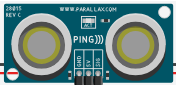
\includegraphics[width=0.4\textwidth]{img/Sensor_distancia.png}
	    \captionof{figure}{Sensor de distancia del guante.}
	    \label{fig:sensdistancia}
	\end{center}

	\item Sensores de fuerza e inclinación, que se visualizan en la Figura \ref{fig:sensfuerzainc}. 

	\begin{center}
	    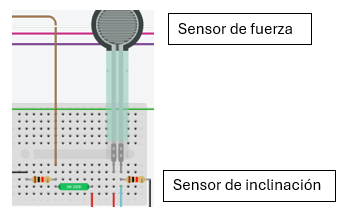
\includegraphics[width=0.6\textwidth]{img/Sensor_fuerza_inclinacion.png}
	    \captionof{figure}{Sensores de fuerza e inclinación.}
	    \label{fig:sensfuerzainc}
	\end{center}
\end{itemize}

El diseño completo del circuito final se puede apreciar en la Figura \ref{fig:guante}. 
\begin{center}
    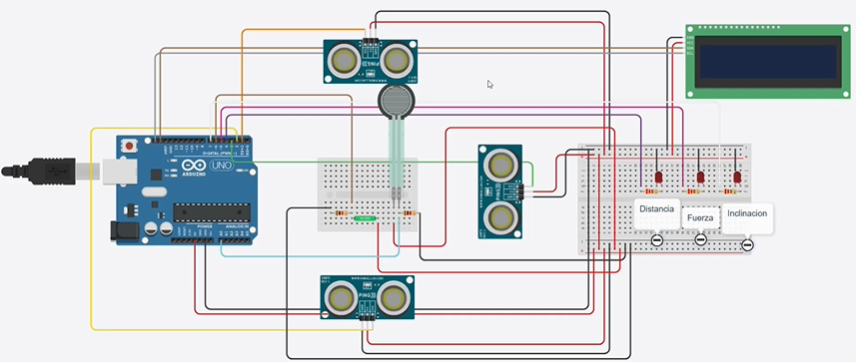
\includegraphics[width=0.9\textwidth]{img/Guante_tinkercad.png}
    \captionof{figure}{Diseño de  \textit{Tinkercad} del guante de detección movimiento involuntarios.}
    \label{fig:guante}
\end{center}


\section{Funcionamiento}
Una vez en funcionamiento, cada vez que la mano excede los límites de los sensores de la caja, la pantalla muestra un mensaje de advertencia que depende cual sea, pone izquierda, derecha o arriba.

También muestra las posibles combinaciones de coincidencias con los datos cargados, como puede ser distancia con fuerza, distancia con inclinación, inclinación con fuerza y muestra un mensaje total cuando se presentan los tres tipos de coincidencias.

Obviamente cuando no se da ningún tipo de coincidencia entre los datos de los sensores y los cargados, la pantalla muestra un mensaje anunciando que todos los valores son correctos.


\section{Presupuesto}
Por último, en la Figura \ref{fig:presguante} ,se ve el presupuesto simplificado del coste de creación y desarrollo de esta herramienta en concreto.
\begin{center}
    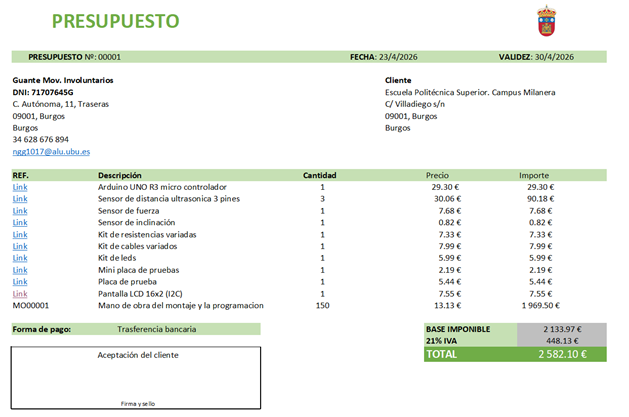
\includegraphics[width=1.0\textwidth]{img/Presupuesto_guante.png}
    \captionof{figure}{Presupuesto del guante de detección de movimientos involuntarios.}
    \label{fig:presguante}
\end{center}